
\chapter{Bibliothèques Scheme}

Pour développer notre approche de modularisation dans le contexte de
systèmes distribués nous avons choisi un langage de programmation nous
permettant de facilement expérimenter avec le code mobile.  Le langage
Termite Scheme, une variante de Scheme étendue avec des
fonctionnalités de programmation distribuée inspirées du langage
Erlang, nous est apparu comme une option intéressante vue sa
performance, sa portabilité et son support pour la méta programmation
facilitée par son homoiconicité.  Notre travail a donc pu se concentrer
sur la conception d'un système de module spécialisé aux besoins du
code mobile.

Ce chapitre introduit la syntaxe de Scheme et les différentes
approches de modularisation existantes.  Afin de faciliter son
adoption, le système de module que nous avons développé se base sur
ces approches.

% Ce concept pose des défis particuliers dans l'implantation.
%Le tout, pour introduire la syntaxe des modules qui permet de résoudre
%les problème avec le code mobile lié mentionné dans le
%chapitre~\ref{ch:mod_sys_dis}.

\section{Scheme et sa syntaxe}

Le langage Scheme\cite{Clinger:2008:SCH:1529966.1529973}, conçu en 1975 par Guy
L. Steele et Gerald Jay Sussman, est une variante minimaliste de Lisp.
Depuis sa conception, plusieurs normes ont vu le jour; les plus connues
étant le R4RS (1991), R5RS (1998), R6RS (2007) et R7RS (2013).

Scheme est un langage de programmation avec un
système de type dynamique.  Les types sont associés aux valeurs plutôt qu'aux
variables et une variable donnée n'est pas contrainte à contenir un type
particulier.  Il permet la programmation fonctionnelle, la programmation
impérative et la méta programmation.

Sur le plan syntaxique, Scheme hérite la
syntaxe préfixe parenthésée de Lisp.  Un programme Scheme est une séquence de
\textit{s-expressions}.  Chaque \textit{s-expression} correspond soit à une
constante, une variable ou une forme \texttt{(\textit{<op>} \textit{<arg>...})}
qui dénote un appel de procédure, un appel de macro, ou une forme spéciale.

Les formes syntaxiques spéciales de base en Scheme sont \lstcode{define}, \lstcode{lambda},
\lstcode{let}, \lstcode{if} et \lstcode{set!}.
\begin{itemize}
  \item La forme \texttt{(define \textit{<name>} \textit{<val>})} associe le nom \textit{<name>} avec
    la valeur de l'expression \textit{<val>}. Il est utilisé pour définir les variables globales.

  \item La forme \texttt{(lambda \textit{<params>} \textit{<body>})} permet la définition de
    procédures anonymes. Les paramètres sont \textit{<params>} et le corps
    de la procédure est l'expression \textit{<body>}.

  \item La forme \texttt{(let \textit{<bindings>} \textit{<body>})} permet de
    créer des associations (\textit{<bindings>}) visibles seulement dans le
    contexte de l'expression \textit{<body>} dont la valeur de la forme
    \texttt{let}. Les associations sont sous la forme d'une liste associative
    nom et valeur.

  %% XXX: Too much???
  \item L'évaluation conditionnelle est obtenue par la forme \texttt{(if
    \textit{<e1>} \textit{<e2>} \textit{<e3>})}.  L'expression \textit{<e2>}
    est exécutée si la valeur de l'expression \textit{<e1>} est vraie sinon
    l'expression \textit{<e3>} est exécutée.

  \item La forme \texttt{(set! \textit{<name>} \textit{<val>})} modifie le contenu de la variable
    \textit{<name>} avec la valeur \textit{<val>}.
\end{itemize}

À titre d'exemple, la figure \ref{fig:fact100} montre un programme Scheme
simple avec deux définitions de fonctions.
\begin{figure}[htbp]
  \begin{tabular}{|l|}\hline
\begin{mplisting}{0.7}
(define sq (lambda (x) (* x x)))

(define fact
  (lambda (n)
    (if (< n 2)
        1
        (* n (fact (- n 1))))))

(println (fact (sq 10)))
\end{mplisting}\\\hline
\end{tabular}

\caption{Programme Scheme qui imprime la factorielle de 100.}

\label{fig:fact100}
\end{figure}


%read from here

%La méta programmation est un paradigme lié à l'utilisation de macros qui sont
%des entités qui manipulent la structure du programme. Elle est utilisée pour
%étendre le langage avec des nouvelles formes syntaxiques pour simplifier l'écriture du code.  La
%section \ref{sec:proc_and_macro} détaille la méta programmation en Scheme.

% Une expression peut être organisé de plusieurs façons, infixe, préfixe ou
% suffixe.  La différence entre ces organisations est l'emplacement de
% l'opération et des opérandes dans l'expression.  Une expression en syntaxe
% infixe place l'opération entre les opérandes.  Cette forme est souvent utilisé
% dans les langages impératif. La forme préfixe commence par l'opérateur suivie
% des opérandes. Cette forme est plus utilisé dans les langages de la famille
% LISP.  La forme suffixe place les opérations après les opérandes.  Le tableau
% \ref{tab:prefix_vs_infix} donne des exemples d'expression préfixe avec
% l'équivalent infixes.


% \begin{verbatim}
% - Scheme
%    - Langage dynamique
%   - Supporte plusieurs paradigmes:
%     - fonctionnel
%     - impérative
%     - méta (programmation de macro)
%   - Préfixé / ~Infixe
%   - S-expression
% \end{verbatim}


%\begin{table}[htbp]
%\begin{center}
%\begin{tabular}{|l|l|}
%  \hline
%  \textbf{Préfixe}& \textbf{Infixe}
%  % & \textbf{Suffixe}
%  \\\hline
%  \begin{mplisting}{0.1}
%(+ 1 2)
%\end{mplisting}&
%  \begin{mplisting}{0.1}
%1 + 2;
%\end{mplisting}
%  % \begin{mplisting}{0.1}
%% 1 2 +
%% \end{mplisting}\\
%\\\hline
%  % \begin{mplisting}{0.22}
%% (proc a1 a2 a3)
%% \end{mplisting}&
%  % \begin{mplisting}{0.22}
%% proc(a1, a2, a3);
%% \end{mplisting}&
%  % \begin{mplisting}{0.22}
%% a1 a2 a3 proc
%% \end{mplisting}\\
%% \hline
%%    \begin{mplisting}{0.25}
%%(if e1
%%    e2
%%    e3)
%%\end{mplisting}&
%%    \begin{mplisting}{0.25}
%%if(e1)
%%  e2;
%%else
%%  e3;
%%\end{mplisting}\\
%%\hline
%\end{tabular}
%\end{center}
%  \caption{Voici un example qui montre une comparaison entre une syntaxe préfixe et infixe.}
%  \label{tab:prefix_vs_infix}
%\end{table}

% La définition des associations globales en Scheme est effectuée avec \lstcode{define}.

Les différents types primitifs disponibles dans la norme Scheme
sont \lstcode{boolean}, \lstcode{pair}, \lstcode{symbol},
\lstcode{number}, \lstcode{char}, \lstcode{string}, \lstcode{vector},
\lstcode{port} et \lstcode{procedure}.
Plusieurs systèmes Scheme offrent des extensions à ces types, tels
les dictionnaires (``hash tables''), les structures (``records'') et tableaux numériques (par exemple Gambit
offre le type \lstcode{u8vector} qui est un tableau d'octets).

\section{Procédures et macros}
\label{sec:proc_and_macro}

Les procédures sont des objets de première classe, c'est-à-dire pouvant
être manipulées comme n'importe quel type de donnée. Elles peuvent
être passées en tant que paramètre à une procédure et retournées en tant que
résultat.  Certaines procédures, comme \lstcode{for-each}, \lstcode{map} et
\lstcode{fold}, en tirent profit.

Les procédures sont définies par la forme \lstcode{lambda} qui a une liste de
paramètres et une séquence d'au moins une \textit{s-expression} comme corps.
Lors de l'appel d'une procédure, chacun des paramètres actuels est évalué puis
propagé à la procédure. C'est un mode de passage de paramètre par valeur. Les
boucles sont normalement exprimées sous la forme de récursion.  Cela est
facilité par l'existence de l'appel terminal garanti.  Il est assez simple
d'ajouter une syntaxe pour les boucles à l'aide de la méta programmation.


% \begin{figure}[ht]
%   \begin{center}
%     \begin{tabular}{|l|}
%       \hline
%     \begin{mplisting}{0.55}
% (define fact
%   (lambda (n) (if (= n 0) 1
%                   (* n (fact (- n 1))))))
% \end{mplisting}\\\hline
%     \end{tabular}
%   \end{center}
%   \label{fig:fact1}
%   \caption{Voici une implémentation de la fonction factoriel en Scheme.
%   Cela montre un exemple de récursion.}
% \end{figure}

% READ Distinguer macro procedure.
% \begin{figure}[ht]
%   \begin{center}
%     \begin{tabular}{|l|}
%       \hline
%     \begin{mplisting}{0.65}
% (define map
%   (lambda (f lst)
%     (if (pair? lst)
%         (cons (f (car lst)) (map f (cdr lst)))
%         lst)))
% \end{mplisting}\\\hline
%     \end{tabular}
%   \end{center}
%   \label{fig:fact1}
%   \caption{Voici une implémentation de la fonction d'ordre supérieur \lstcode{map} en Scheme.
%   Cela montre un exemple utilise les procédure en objets de première classe et
%   aussi un exemple d'application récursive.}
% \end{figure}



% La récursion est la façon dont les boucle sont faites.
La méta programmation en Scheme est basée sur la capacité d'un programme de
manipuler d'autre programme comme des données. Cela implique qu'il est possible
de générer, analyser et modifier le code d'un autre programme.  Les
constructions utilisées pour manipuler le code du programme et ajouter des
extensions au langage sont les macros.

En C et C++, les macros sont basées sur un modèle de remplacement textuel simple
et ne permettent pas de récursion se référant à elle-même.  Un appel à la macro
est remplacé par le corps de celle-ci. Les macros de style Lisp permettent des
transformations qui se font avec
l'ensemble des procédures du langage, ce qui leur donne plus de flexibilité.  La
différence entre les procédures et les macros est le mode de passage de
paramètres.  Les paramètres sont passés à la macro sans être évalués.
Certaines implémentations de Scheme offrent la forme \lstcode{define-macro}
pour définir les macros.  Cette forme est équivalente au \lstcode{defmacro} de
Lisp. Elle accepte en entrée des \textit{s-expression}s et retourne une
\textit{s-expression}.

\begin{figure}[htbp]
  \begin{tabular}{|l|}\hline
\begin{mplisting}{0.7}
(define-macro (include filename)
  (call-with-input-file
    filename
    (lambda (port)
      `(begin
        ,@(read-all port)))))
\end{mplisting}\\\hline
\end{tabular}

  \caption{Implémentation de la macro \texttt{include} qui permet l'inclusion
  d'un fichier dans un autre fichier avec la forme \texttt{define-macro}.}

  \label{fig:macro_include}
\end{figure}

Un exemple qui montre les capacités des macros Scheme est la macro
\lstcode{include}.  Cette macro permet l'inclusion du contenu d'un fichier au
point d'appel.  Pour inclure un fichier dans un autre, il faut tout d'abord
lire le contenu du fichier à inclure. Ensuite, il suffit de retourner le code
lu. La figure \ref{fig:macro_include} montre une implémentation de cette macro
avec \lstcode{define-macro}.  Pour les systèmes Scheme n'offrant pas la forme
\lstcode{define-macro}, il est assez simple d'implémenter la forme
\lstcode{include} avec \lstcode{define-syntax} qui est une forme de définition
de macro alternative à \lstcode{define-macro}. L'implémentation de cette macro
est donnée à la figure \ref{fig:macro_include_def_syntax}. Les particularités
de \lstcode{define-syntax} ne sont expliquées puisqu'elles ne sont pas
pertinentes à ce mémoire.

% --------------------------------------MOVE--------------------------------------

% Certaines implémentations de Scheme n'ont pas la forme
% \lstcode{define-macro}. Il est possible d'écrire la macro
% \lstcode{include} en utilisant la \lstcode{define-syntax}
% et \lstcode{syntax-case} qui fait partie du standard R5RS
% \cite{Scheme:R5RS}. La figure \ref{fig:macro_include_def_syntax}
% montre implémentation possible de cette macro.

\begin{figure}[ht]
\begin{tabular}{|l|}\hline
\begin{mplisting}{0.8}
(define-syntax include
  (lambda (stx)
    (syntax-case stx ()
      ((_ filename)
       (let ((content
               (call-with-input-file
                  (syntax->datum (syntax filename))
                  (lambda (port)
                    `(begin ,@(read-all port))))))
         (datum->syntax stx content))))))
\end{mplisting}\\\hline

\end{tabular}
   \caption{Implémentation de la macro \texttt{include} qui permet l'inclusion
   d'un fichier dans un autre fichier avec la forme \texttt{define-syntax}.}

   \label{fig:macro_include_def_syntax}
\end{figure}

\section{Structure des bibliothèques}

Les bibliothèques, aussi appelées modules, facilitent le partage de
fonctionnalités entre plusieurs programmes. Dans le standard
R4RS\cite{Scheme:R4RS} et R5RS\cite{Scheme:R5RS} les modules consistent en des
fichiers Scheme qui contiennent des définitions de procédures et de macros. Ils
sont chargés dans l'environnement global par la procédure \lstcode{load}. Certaines
implémentations de Scheme ont la forme spéciale \lstcode{include} qui permet de
séparer un module Scheme en plusieurs parties. Cette forme peut s'ajouter
facilement au langage (tel que montré à la figure
\ref{fig:macro_include_def_syntax}).  Le modèle de bibliothèque basé sur
\texttt{load} et \texttt{include} possède plusieurs lacunes.

%% Gambit doc
\begin{itemize}
  \item Ce modèle de chargement n'est pas à l'abri des chargements multiples
    d'un module qui mène soit à de la duplication de code (dans le cas de la forme \lstcode{include})
    ou à de la réévaluation d'un code (dans le cas de \lstcode{load}).

  \item Toutes les déclarations dans un module sont ajoutées à l'environnement
    global lors du chargement par \lstcode{load}. Cela mène à des conflits de
    nom entre les identifiants du module principal et des modules importés.

  \item L'importation d'un module par \lstcode{load} ou \lstcode{include} nécessite la connaissance
    de son emplacement dans le système de fichier.

\end{itemize}

% \begin{verbatim}
% +-----------------------------------+
% | - Analyse lexicale                |
% | - Analyse syntaxique              |
% | - Expansion macro                 |
% | - Evaluation                      |
% +-----------------------------------+
% \end{verbatim}

Le chargement d'un module dans Gambit Scheme par \lstcode{load} se fait en plusieurs
phases: l'analyse lexicale, l'analyse syntaxique, l'expansion de macro et
l'évaluation. L'analyse lexicale brise l'expression en lexèmes. La séquence de
lexèmes est associée à un contexte par l'analyse syntaxique dans laquelle il y a aussi
une expansion des macros. L'inclusion d'un fichier avec \lstcode{include} n'effectue qu'une
analyse lexicale qui est effectuée par la procédure \lstcode{read-all}. L'évaluation
est effectuée après l'analyse syntaxique et l'expansion des macros. D'autres systèmes
Scheme permettent le chargement des macros par \lstcode{load}.

Dans un module, il y a du code qui est exécuté lors de l'expansion (les macros)
et à l'évaluation. La procédure \lstcode{load} donne accès aux procédures définies
dans le module, mais pas aux macros, car elles sont expansées.  Après un
\lstcode{load}, il ne reste que les procédures et variables globales qui
résultent de l'expansion des macros.  Pour avoir accès aux macros, il faut
utiliser la forme spéciale \lstcode{include} qui est expansée par le contenu du
fichier.  L'expression \lstcode{(include "foo.scm")} est remplacée par le
contenu du fichier \lstcode{foo.scm}. L'exemple \ref{fig:r4rs_fact} montre un
exemple de module simple n'utilisant que la procédure \lstcode{load}.

\begin{figure}[ht]
  \begin{center}
    \begin{tabular}{|l|l|}
    \hline
    \begin{mplisting}{0.4}
;; fact.scm
(define (fact n)
  (if (< n 2)
    n
    (* n (fact (- n 1)))))
\end{mplisting} &
    \begin{mplisting}{0.4}
;; main.scm
(load "fact.scm")
(display (fact 5))
\end{mplisting} \\\hline
    \end{tabular}
  \end{center}

  \caption{Le fichier \texttt{fact.scm} est un exemple de module R4RS exposant
  la fonction mathématique \lstcode{fact}. Le fichier \texttt{main.scm} est un
  programme principal qui utilise le module \texttt{fact.scm}.}
  \label{fig:r4rs_fact}
\end{figure}


% - Structure global
% - Nom module
% - Export
% - Import
% - Corps de module

Le standard R6RS\cite{Scheme:R6RS} renforce le concept de module avec la
syntaxe \lstcode{library}.  Un module R6RS est séparé en 4 parties: le nom, une
sous-forme \lstcode{export}, une sous-forme \lstcode{import} et le corps du
module. Le nom du module l'identifie de façon unique, il peut contenir une
spécification de version. La version est spécifiée par une liste d'entiers
positifs. Une liste vide \lstcode{()} correspond à ne pas spécifier la
version. Ensuite, il y a la liste des exportations qui est spécifiée par la sous-forme
\lstcode{export}. Chaque élément de cette liste est soit un identifiant ou une
sous-forme \lstcode{rename} qui renomme l'identifiant exporté.
L'\lstcode{import} donne la liste des dépendances du module. Chaque dépendance
spécifie:

\begin{itemize}
  \item le nom du module importé et de façon optionnelle, une contrainte sur
    la version;
  \item le niveau d'import (temps d'expansion de macros ou évaluation);
  \item un sous-ensemble de l'\lstcode{export} du module et le nom local
    utilisé au sein du module présent pour chaque exportation du module.
\end{itemize}

Le corps du module contient une séquence de définitions suivie par une séquence
d'expressions. Une définition peut être locale ou exportée. Les expressions
initialisent le module lors de l'exécution.  Le R6RS ajoute aussi la forme
\lstcode{import} pour l'importation d'un module et enlève la procédure
\lstcode{load}.  Contrairement au \lstcode{load}, la forme \lstcode{import}
garantit le chargement unique d'un module.  La syntaxe du \lstcode{import}
permet de manipuler les noms des symboles importés et exportés.\\
\begin{figure}[ht]
  \lstset{language={scheme},
          frame=single}
  \begin{mplisting}{0.5}
(library <library name>
  (export <export spec> ...)
  (import <import spec> ...)
  <library body>)
\end{mplisting}
  \caption{Structure globale d'un module R6RS}
\end{figure}

La forme \lstcode{import} de R6RS permet l'importation d'un ensemble de modules.
Chaque spécification d'import \lstcode{<import spec>} peut être une simple
importation ou une importation avec un niveau. Les différents niveaux d'importation sont:
\lstcode{run}, \lstcode{expand} ou \lstcode{(meta <level>)}.  Le niveau méta
donné par \lstcode{<level>} est un entier exact. Un niveau d'importation 0
correspond à \lstcode{run} et un niveau d'importation de 1 correspond à
\lstcode{expand}.

% L'importation d'un module contient les sous formes suivantes:
% \begin{center}
% \begin{mplisting}{0.7}
%   <libref>
%   (library <libref>)
%   (only <import set> <identifier_1> ...)
%   (except <import set> <identifier_1> ...)
%   (prefix <import set> <identifier>)
%   (rename <import set> (<identifier_1> <identifier_2>))
% \end{mplisting}
% \end{center}

% \begin{itemize}
%   \item \lstcode{(rename  (<identifier1> <identifier_2>))}
% \end{itemize}

La syntaxe pour l'importation avec les niveaux méta est décrite dans la
spécification R6RS~\cite{Scheme:R6RS}. Le \lstcode{import} R6RS permet un grand
contrôle lors de l'importation des modules au prix d'une sémantique plus complexe.

Les déclarations d'un module R6RS sont dans un espace distinct de l'espace global et
des autres modules. Les déclarations d'un module ne peuvent pas être en conflit avec
des déclarations globales ou d'autres modules. L'élément qui permet de distinguer deux modules
est leurs identifications (nom avec version). Le nom du module correspond à l'espace de nom du module.
C'est ce qui unit les déclarations au module et empêche les conflits de nom entre
les modules.


%Cette syntaxe
%est fortement lié à ce module. Chaque module a son propre
%espace de environnement. dans l'espace de nom du module sert d'espace de nom pour les associations
%du module. Ce modèle introduit le concept d'espace de nom
%qui donne l'appartenance des fonctionnalités à un module. Cela règle le
%problème que module redéfinisse les fonctionnalités d'un autre module.


% Le concept de bibliothèque a été raffiné  dans le R6RS.  Le R6RS rend le
% support de la procédure \texttt{load} optionnel et ajoute une forme spéciale
% \texttt{library} pour définir des bibliothèques et une autre forme spéciale
% \texttt{import} pour gérer la inclure une bibliothèque.  Les noms utilise
% pour nommer une bibliothèque peuvent seulement contenir des symboles et des
% numéros de versions à la fin. Les expression import et export doivent seulement
% apparaître une seul fois dans le définition de la bibliothèques.

% Les bibliothèques ainsi définit, lie chaque définitions à la bibliothèque.  Cela
% permet la réutilisation des mêmes identificateurs dans deux bibliothèque
% différente.  Les conflits de nom sont gérés lors de l'importation des la
% bibliothèques. L'importation d'un module est permit au sein d'une bibliothèque
% comme dans un programme principale. La syntaxe d'un import reste identique dans
% ce deux cas.

% Pour évité ces conflit, il faut que tous les noms utilisés au sein des
% bibliothèques soit distinct, ce qui ajoute une tâche au programmeur.

% What is define-library?
Le standard R7RS\cite{Scheme:R7RS} simplifie la syntaxe des modules
R6RS\cite{Scheme:R6RS}.  L'importation d'un module fait abstraction du niveau
d'importation. Les macros et les procédures sont importées de façon
transparente. La procédure \lstcode{load} est conservée. La forme spéciale pour
définir un module est \lstcode{define-library}. Il n'y a pas d'ordre spécifique
dans les déclarations de la bibliothèque comme en R6RS. Un module R7RS commence par
un nom suivi de plusieurs déclarations.\\
\begin{figure}[ht]
  \centering
  \lstset{language={scheme},frame=single}
  \begin{mplisting}{0.5}
(define-library <library name>
  <library declaration>*)
\end{mplisting}
  \caption{Structure globale d'un module R7RS}
  \label{fig:syntax->define-library}
\end{figure}

Une déclaration dans un module est soit un \lstcode{import}, un \lstcode{export},
un \lstcode{include}, un \lstcode{include-ci}, un \lstcode{cond-expand} ou un
bloc \lstcode{begin}.
\begin{itemize}
  \item La déclaration \lstcode{import} est équivalente au R6RS sans le concept
    de niveau d'importation.

  \item La déclaration \lstcode{export} est idem au R6RS.

  \item Les déclarations \lstcode{include} et \lstcode{include-ci} permettent
    l'inclusion d'un fichier en tant qu'un bloc de code.  La seconde forme
    non sensible à la casse des caractères.

  \item La déclaration \lstcode{cond-expand} est une extension du
    \texttt{SRFI-0}~\cite{SRFI-0} dans le contexte d'une bibliothèque
    permettant l'inclusion conditionnelle de code.

\end{itemize}

La forme \lstcode{import} en R7RS permet d'importer un ensemble d'identifiants
qui sont exportés par un module. Chaque ensemble importé spécifie le nom des
identifiants du module et parfois même associe un nom local aux identifiants.
L'\lstcode{import} peut prendre l'une des formes suivantes:
\begin{itemize}
  \label{itm:import-set}
  \item \texttt{\textit{<library-name>}}
  \item \texttt{(only \textit{<import-set>} \textit{<id1>} ...)}
  \item \texttt{(except \textit{<import-set>} \textit{<id1>} ...)}
  \item \texttt{(prefix \textit{<import-set>} \textit{<id>})}
  \item \texttt{(rename \textit{<import-set>} (\textit{<id1>} \textit{<id2>}) ...)}
\end{itemize}


Dans la première forme, tous les identifiants exportés par
la bibliothèque \texttt{\textit{<library-name>}} sont importés.
Les autres types de \texttt{\textit{<import-set>}} modifient
l'ensemble comme suit:
\begin{itemize}
  \item \textbf{only} inclut seulement les identifiants spécifiés. C'est une
    erreur d'importer un identifiant non exporté par la bibliothèque.

  \item \textbf{except} permet d'exclure des identifiants de l'ensemble.

  \item \textbf{rename} renomme les identifiants importés.

  \item \textbf{prefix} ajoute un préfixe à l'ensemble des identifiants
    importés.
\end{itemize}

% L'implémentation des bibliothèques Scheme est basé sur le standard R7RS qui
% conserve la procédure \texttt{load} que le R6RS enlève et remplace la structure
% des bibliothèques.  Une bibliothèque en R7RS remplace la forme
% \lstcode{library} par \texttt{define-library}. Ces deux formes ont beaucoup de
% similarité, il existe une méthode pour transformer certaines bibliothèques R6RS
% en bibliothèques R7RS. Takashi Kato a publié un article au \emph{Scheme
% Workshop} 2014 qui explique une procédure pour écrire un module R6RS en R7RS
% \cite{SW2014:R6RS/on/R7RS}.  L'extension de fichier utilisé par les définitions
% des bibliothèques est \verb|.sld| qui signifie \emph{Scheme Library
% Declaration}.

\begin{center}
  \begin{figure}[h]
  \begin{tabular}{|l|l|}
    \hline
    \begin{mplisting}{0.5}
;; Bibliotheque R6RS
(library (math)
  (export fact)
  (import (rnrs base))
  (define (fact n)
    (if (< n 2)
      1
      (* n (fact (- n 1))))))
\end{mplisting} &
    \begin{mplisting}{0.5}
;; Bibliotheque R7RS
(define-library (math)
  (export fact)
  (import (scheme base))
  (begin
    (define (fact n)
      (if (< n 2)
        1
        (* n (fact (- n 1)))))))
\end{mplisting}\\\hline
  \end{tabular}
    \caption{Comparaison entre la syntaxe des modules R6RS et R7RS}
% \caption{À gauche, il y a un exemple d'une bibliothèque mathématique dans le format R6RS qui implémente
% la fonction factoriel. À droite, une réécriture de la bibliothèque de gauche en R7RS.}
  \label{fig:r6rs_r7rs_math_mdoule}
\end{figure}
\end{center}


\section{Conclusion}
%
Pour notre objectif de modularisation dans les systèmes distribués, les
révisions de Scheme qui offrent les fonctionnalités requises sont R6RS et R7RS.
Elles permettent toutes les deux la modularisation du code et la création de
modules avec des noms uniques, ce qui est requis pour le bon fonctionnement du
code mobile.   Nous avons choisi l'approche avec \lstcode{define-library},
puisque Gambit se veut compatible avec le R7RS. Cela a permis d'expérimenter
avec le code mobile. En plus, cela facilite son adoption et sa portabilité
entre les implémentations de Scheme qui sont de plus en plus compatibles avec
R7RS.


% - (import (foo)) ; exportant f1 f2 f3
% ===>
% - (##demand-module foo)
% - (##namespace ("foo") f1 f2 f3)
% - macros
% - (##namespace (""))




%% ---- MOVED to chapter 4 ----

%\section{Chargement des bibliothèques}

%Un système est composé d'un ensemble d'éléments (modules) qui interagissent
%entre eux.  Une bibliothèque fait office de module au sein d'un système simple
%ou complexe.
%%La collection des modules s'effectue au sein d'un

%% TODO: voir chargé
%Le chargement d'une bibliothèque Scheme (ou module) est séparé en plusieurs niveaux.
%% TODO: later
%Les bibliothèques sont soit lu du disque vers la mémoire durant l'exécution
%ou déjà dans la mémoire du processus. Durant la compilation les modules sont
%collecté pour construire un exécutable. Le chargement
%d'une bibliothèque inclut une phase de recherche sur le système de fichier pour valider
%l'existence de la bibliothèque et des fonctionnalités demandés. L'emplacement des
%bibliothèques sur le système de fichier est lié par défaut aux chemin spécifié par
%le \lstinline{##module-search-order} a comme défaut \lstinline{~~lib} et \lstinline{~~userlib}.


%La procédure exacte de chargement des bibliothèques par \verb|import|
%n'est pas spécifier par le standard R7RS. Le standard spécifie seulement la syntaxe
%à utilisé et le de comportement principal qui est
%requis. L'importation d'une bibliothèque doit chargé la bibliothèque
%et rendre c'est fonctionnalité disponible dans le contexte
%l'importation a eu lieu qui peut soit ovenir d'un programme principale
%ou d'une bibliothèque.

%Le chargement d'une bibliothèque peut-être effectuée à l'exécution par
%l'utilisation de \texttt{eval} (par \texttt{load}) pour les fichiers source et
%\texttt{load-objcet-file} pour les bibliothèques compilées. Cette recherche
%peut aussi avoir lieu durant l'édition des lien en utilisant les méta-infos
%contenus dans les \textbf{.c} qui sont chacun compilé par le compilateur C
%en \textbf{.o} et lié par le \textit{linker}.

%\section{Modèle dynamique}
%Dans ce modèle les bibliothèques sont lié au programme durant l'exécution. Cela
%nécessite que les bibliothèques soit organisé sur le système de fichier d'une façon
%distingable. Chaque module doit posséder un nom unique qui permet d'y référer.
%Ce nom unique va être utilisé lors de la collection des dépendances.


%%Les bibliothèques
%%sont soit en code source ou compilé nativement avec l'extension (\textit{.oN})
%%où le N correspond à la version du binaire qui commence à 1.


%La recherche des bibliothèques est effectué dans un ordre spécifique
%indépendant de la spécification.  L'algorithme de recherche les bibliothèques
%prend entré le nom de la bibliothèque et retourne le chemin absolu
%correspondant à sont emplacement dans l'arborescence du système de fichier. Les
%bibliothèques sont situées dans différents répertoires l'origine du programme,
%le répertoire des bibliothèques système (\lstinline{~~lib}) et le
%répertoire de bibliothèque utilisateur (\lstinline{~~userlib}).

%% \begin{itemize}
%%   %% XXX: directory where the executable is located (usefull for devel no need to install the module). collecté
%%   \item \verb|origin/dummy.sld|
%%   \item \verb|origin/dummy/dummy.sld|
%%   \item \verb|~~userlib/dummy.sld|
%%   \item \verb|~~userlib/dummy/dummy.sld|
%%   \item \verb|~~lib/dummy.sld|
%%   \item \verb|~~lib/dummy/dummy.sld|
%% \end{itemize}

%Chaque module possède trois niveau d'initialisation dans le système numéroté de
%0 à 2. Le niveau 0 indique que le module n'a pas été initialisé. Ces les niveau
%des module qui ont juste été collecté par le système. Le niveau 1 indique que
%le descripteur du module à été récupéré. L'étape 2 est utilisé pour indiquer
%les module chargé.

%Soit un système avec les dépendance suivante:
%\begin{figure}[ht]
%  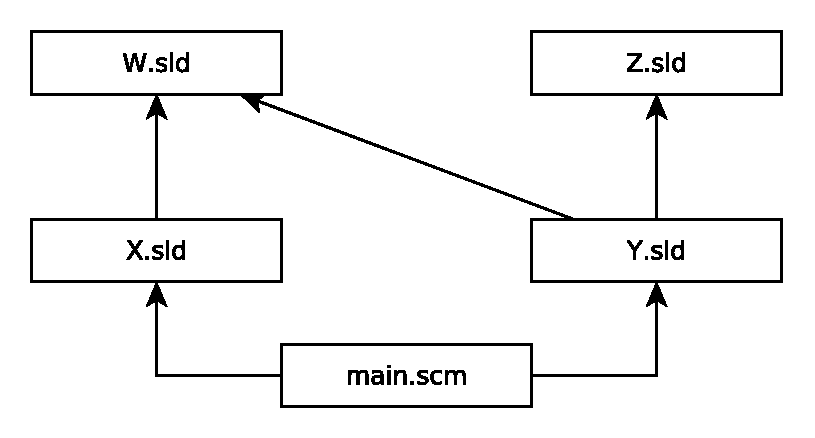
\includegraphics{figures/system-example}
%  \caption{Un exemple d'un système fictif composé de différents modules.
%  Le module principale se nomme utilise l'extension \textbf{.scm}
%  et les bibliothèques porte l'extension \textbf{.sld}}
%\end{figure} % TODO: use yed for that graph


%Le démarrage du module principal Main.scm déclenche la collection des modules X
%et Y, qui récursivement déclenche la collection de W et Z. L'algorithme de
%collection des modules ignore les module qui apparaisse plusieurs fois au sein
%du graphe.

%Une fois la collection de tous ces modules est complété le descripteur de
%module est récupéré par un appels à \verb|dlopen| et \verb|dlsym| dans le cas
%compilé.


%\section{Module hébergé}

%Un module qui est hébergé est un module qui dont son contenu
%se retrouve sur un domain comme \url{github.com}.


%\begin{figure}[ht]
%\begin{lstlisting}
%hostname      = +( domainlabel "." ) toplabel
%domainlabel   = alphanum | alphanum *( alphanum | "-" ) alphanum
%toplabel      = alpha | alpha *( alphanum | "-" ) alphanum
%alphanum      = alpha | digit
%alpha         = [a-zA-Z]
%digit         = [0-9]
%\end{lstlisting}
%  \caption{Grammaire BNF représentant un hostname selon un sous
%  ensemble du RFC-2396.}
%\end{figure}

%La différence avec la spécification du hostname dans le RFC-2396
%est que le hostname ne peut pas finir par un point et doit contenir
%au moins un \verb|domainlabel|. C'est pour permettre de distingué
%un module local et un module hébergé.

%\subsection{Module gambit/git}

%Ce module offre un interface pour utiliser interagir avec les des dépôts git.
%Il permet de cloner un dépôts qui est hébergé sur \url{github.com}. Un clone du
%dépôts est simplement un copie qui contient les informations suffisantes pour
%passer d'une version d'un module à un autre. L'opération qui permet de changer
%de version est \emph{checkout}.


%%-------------------------------------------------------------------------------
%%
%%Modèle "link dynamique" :
%%  recherche des libs au run time, utilisation de eval (par load) et
%%  load-object-file
%%
%%  % gsi main.scm      ou      % gsc main.scm ; gsi main.o1
%%
%%    origin/main.scm    : (import X Y)
%%          /X/X.sld     : (import)
%%
%% ~~userlib/Y/Y.sld     : (import Z)
%%
%%     ~~lib/Z/Z.sld     : (import)
%%          /Z.o1
%%
%%-------------------------------------------------------------------------------
%%
%%Modèle "link statique" :
%%  recherche des libs au link time en utilisant les méta-infos
%%  dans les .c (demand-lib et supply-lib), chaque .c compilé en
%%  un .o séparément et les .o linkés par le compilateur C
%%
%%  % gsc -obj -keep-c X.sld      ;; créer .c et .o
%%  % gsc -obj -keep-c Y.sld      ;; créer .c et .o
%%  % gsc -obj -keep-c Z.sld      ;; créer .c et .o
%%  % gsc -obj -keep-c main.scm   ;; créer .c et .o
%%  % gsc -exe main.c             ;; combine les .o pour créer main.exe
%%
%%    origin/main.scm    : (import X Y)
%%          /main.c      : (demand-lib X Y)
%%          /main.o
%%          /X/X.sld     : (import)
%%            /X.c       : (demand-lib) (supply-lib X)
%%            /X.o
%%
%% ~~userlib/Y/Y.sld     : (import Z)
%%          /Y/Y.c       : (demand-lib Z) (supply-lib Y)
%%          /Y/Y.o
%%
%%     ~~lib/Z/Z.sld     : (import)
%%          /Z/Z.c       : (demand-lib) (supply-lib Z)
%%          /Z/Z.o
%%
%%-------------------------------------------------------------------------------
%%
%%Modèle "whole-program" :
%%  recherche des libs au compile time en utilisant les imports
%%  dans les fichiers sources, les AST de toutes les libs fusionnées
%%  en un seul AST compilé par gsc (donc un seul .c généré et compilé
%%  par le compilateur C pour créer main.exe)
%%
%%  % gsc -exe -whole-program main.scm
%%
%%    origin/main.scm    : (import X Y)
%%          /X/X.sld     : (import)
%%
%% ~~userlib/Y/Y.sld     : (import Z)
%%
%%     ~~lib/Z/Z.sld     : (import)
%%
%%-------------------------------------------------------------------------------
%% correction d’une petite coquille…
%% /Y.c       : (demand-lib Z) (supply-lib Y)
%% /Y.o
%%
%% ~~lib/Z/Z.sld     : (import)
%% /Z.c       : (demand-lib) (supply-lib Z)
%% ...


%% (check-sld "/tmp/scheme/base/base.sld" "/tmp/scheme/base")
%% (check-sld "/tmp/scheme/base.sld" "/tmp/scheme")
%% (check-sld
%%  "/home/frederic/Documents/MasterResearch/gambit9/lib/cocolappin/scheme/base/base.sld"
%%  "/home/frederic/Documents/MasterResearch/gambit9/lib/cocolappin/scheme/base")
%% (check-sld
%%  "/home/frederic/Documents/MasterResearch/gambit9/lib/cocolappin/scheme/base.sld"
%%  "/home/frederic/Documents/MasterResearch/gambit9/lib/cocolappin/scheme")
%% (check-sld
%%  "/home/frederic/Documents/MasterResearch/g9/lib/scheme/base/base.sld"
%%  "/home/frederic/Documents/MasterResearch/g9/lib/scheme/base")
%% object-file-path: /home/frederic/Documents/MasterResearch/g9/lib/scheme/base/.gambit_409003@C/base.o1
%% ("/home/frederic/Documents/MasterResearch/g9/lib/scheme/base/base.sld"
%%  .
%%  #<input-port #2 "/home/frederic/Documents/MasterResearch/g9/lib/scheme/base/base.sld">)
